% THIS IS SIGPROC-SP.TEX - VERSION 3.1
% WORKS WITH V3.2SP OF ACM_PROC_ARTICLE-SP.CLS
% APRIL 2009
%
% It is an example file showing how to use the 'acm_proc_article-sp.cls' V3.2SP
% LaTeX2e document class file for Conference Proceedings submissions.
% ----------------------------------------------------------------------------------------------------------------
% This .tex file (and associated .cls V3.2SP) *DOES NOT* produce:
%       1) The Permission Statement
%       2) The Conference (location) Info information
%       3) The Copyright Line with ACM data
%       4) Page numbering
% ---------------------------------------------------------------------------------------------------------------
% It is an example which *does* use the .bib file (from which the .bbl file
% is produced).
% REMEMBER HOWEVER: After having produced the .bbl file,
% and prior to final submission,
% you need to 'insert'  your .bbl file into your source .tex file so as to provide
% ONE 'self-contained' source file.
%
% Questions regarding SIGS should be sent to
% Adrienne Griscti ---> griscti@acm.org
%
% Questions/suggestions regarding the guidelines, .tex and .cls files, etc. to
% Gerald Murray ---> murray@hq.acm.org
%
% For tracking purposes - this is V3.1SP - APRIL 2009

\documentclass{acm_proc_article-sp}

\makeatletter
\def\@copyrightspace{\relax}
\makeatother

\usepackage{hyperref}
\hypersetup{
     colorlinks   = true,
     citecolor    = cyan
}
\usepackage{bbm}
\usepackage{dsfont}

\begin{document}

\title{Abstract Classification
% \titlenote{(Does NOT produce the permission block, copyright information nor page numbering). For use with ACM\_PROC\_ARTICLE-SP.CLS. Supported by ACM.}
}
\subtitle{[COMP 598 Group Project 2]
\titlenote{The complete dataset of this report is available at
\texttt{http://www.acm.org/eaddress.htm}
\\\\
The implementation of the algorithm described in this report is avaiable at
\texttt{http://www.acm.org/eaddress.htm}}}
%
% You need the command \numberofauthors to handle the 'placement
% and alignment' of the authors beneath the title.
%
% For aesthetic reasons, we recommend 'three authors at a time'
% i.e. three 'name/affiliation blocks' be placed beneath the title.
%
% NOTE: You are NOT restricted in how many 'rows' of
% "name/affiliations" may appear. We just ask that you restrict
% the number of 'columns' to three.
%
% Because of the available 'opening page real-estate'
% we ask you to refrain from putting more than six authors
% (two rows with three columns) beneath the article title.
% More than six makes the first-page appear very cluttered indeed.
%
% Use the \alignauthor commands to handle the names
% and affiliations for an 'aesthetic maximum' of six authors.
% Add names, affiliations, addresses for
% the seventh etc. author(s) as the argument for the
% \additionalauthors command.
% These 'additional authors' will be output/set for you
% without further effort on your part as the last section in
% the body of your article BEFORE References or any Appendices.

\numberofauthors{3} %  in this sample file, there are a *total*
% of EIGHT authors. SIX appear on the 'first-page' (for formatting
% reasons) and the remaining two appear in the \additionalauthors section.
%
\author{
% You can go ahead and credit any number of authors here,
% e.g. one 'row of three' or two rows (consisting of one row of three
% and a second row of one, two or three).
%
% The command \alignauthor (no curly braces needed) should
% precede each author name, affiliation/snail-mail address and
% e-mail address. Additionally, tag each line of
% affiliation/address with \affaddr, and tag the
% e-mail address with \email.
%
% 1st. author
\alignauthor
Benedicte Leonard-Cannon\\
  \affaddr{McGill University}\\
       %\affaddr{1932 Wallamaloo Lane}\\
      % \affaddr{Wallamaloo, New Zealand}\\
       \email{teabennie@gmail.com}       
% 2nd. author
\alignauthor
Faiz Khan \\
 \affaddr{McGill University}\\
      % \affaddr{P.O. Box 1212}\\
      % \affaddr{Dublin, Ohio 43017-6221}\\
       \email{dridon@gmail.com }
% 3rd. author
\alignauthor Sherry Shanshan Ruan\\
       \affaddr{McGill University}\\
      % \affaddr{1 Th{\o}rv{\"a}ld Circle}\\
     %  \affaddr{Hekla, Iceland}\\
     \email{sherry.s.ruan@gmail.com}
%\and  % use '\and' if you need 'another row' of author names
%% 4th. author
%\alignauthor Lawrence P. Leipuner\\
%       \affaddr{Brookhaven Laboratories}\\
%       \affaddr{Brookhaven National Lab}\\
%       \affaddr{P.O. Box 5000}\\
%       \email{lleipuner@researchlabs.org}
%% 5th. author
%\alignauthor Sean Fogarty\\
%       \affaddr{NASA Ames Research Center}\\
%       \affaddr{Moffett Field}\\
%       \affaddr{California 94035}\\
%       \email{fogartys@amesres.org}
%% 6th. author
%\alignauthor Charles Palmer\\
%       \affaddr{Palmer Research Laboratories}\\
%       \affaddr{8600 Datapoint Drive}\\
%       \affaddr{San Antonio, Texas 78229}\\
%       \email{cpalmer@prl.com}
}
% There's nothing stopping you putting the seventh, eighth, etc.
% author on the opening page (as the 'third row') but we ask,
% for aesthetic reasons that you place these 'additional authors'
% in the \additional authors block, viz.
%\additionalauthors{Additional authors: John Smith (The Th{\o}rv{\"a}ld Group,
%email: {\texttt{jsmith@affiliation.org}}) and Julius P.~Kumquat
%(The Kumquat Consortium, email: {\texttt{jpkumquat@consortium.net}}).}
\date{30 July 1999}
% Just remember to make sure that the TOTAL number of authors
% is the number that will appear on the first page PLUS the
% number that will appear in the \additionalauthors section.

\maketitle
\begin{abstract}
TBD
\end{abstract}

%% A category with the (minimum) three required fields
%\category{H.4}{Information Systems Applications}{Miscellaneous}
%%A category including the fourth, optional field follows...
%\category{D.2.8}{Software Engineering}{Metrics}[complexity measures, performance measures]
%
%\terms{Theory}
%
%\keywords{ACM proceedings, \LaTeX, text tagging} % NOT required for Proceedings


%-------------------------------------- Introduction  --------------------------------------%
\section{Introduction}
In text classification we aim at building predictors that classify text documents into a specific category from a given set. Typically this is done by taking an input of text documents and labels for the categories and using those train classifiers to be able to predict those text documents. Our use case specifically deals with classifying an input set of approximately 96,000 abstracts that are labelled as either being from cs, stat, math or physics fields. 

In order to use standard classifiers for these situations we first need to transform the text in to inputs that may be used with standard machine learning algorithms. Many feature engineering strategies such as bag-of-words, bi-grams and n-grams are available. We employed the bag-of-words strategy in the construction of our feature set. 

In preprocessing we tokenize our data using two lexers. We then run a series of filters and transformations. We calculate the number of occurrence of all the words and drop all of the words that occur less than five times in order to cater to limited computational resources. We select our features using univariate feature selection to get the 2,000 words with highest variance using chi-squared. We do this twice, once using stemming and once without. We then generate four datasets with the 2,000 words, binary with/without stemming and bag-of-words with/without stemming. The binary set simply sets a 1 if the word occurs otherwise it leave it at 0 and the bag-of-word sets show the number of occurrences in the abstracts. 

We trained our input on three classifiers. We used our own implementation of Naive Bayes, K nearest neighbours along with the scikit-learn's Random Forest implementation. We ran a 5-fold cross validation on these classifiers to tune the parameters and then tested them on a testing set kept separate from the validation step. 

There are several use cases for these classifiers. Online journal publishers such as ACM could use these classifiers to auto-classify documents to their respective categories. Search Engines such as Google Scholar could use these classifiers to match keywords to the relevant articles. Finally, journals could expand the categories and use similar classifiers to match new paper submissions to relevant fields the most appropriate reviewers in the field. 







%-------------------------------------- Related work --------------------------------------%
\section{Related Work}
In the following section, we present existing work conducted by other researchers in the task of text categorization.

Genkin and Lewis \cite{citeulike:1472197} proposed a Bayesian lasso logistic regression model for binary text categorization that relied on a Laplace prior to reduce the risk of overfitting. Their approach addressed the impracticality of fitting a standard logistic regression model to a dataset containing a large feature space. More precisely, their training algorithm used prior probability distributions of the model parameters to encourage model sparsity. According to them, this approach produced a compact model that is effective and does not overfit. In practice, their algorithm performed as well as two state-of-the-art categorization models (support vector machines (SVM) and ridge logistic regression) on five standard test sets (ModApte, RCV1-v2, OHSUMED, WebKB and 20 NG). 

Joachims \cite{joachims98a} was the first to study the performance of SVMs for text classification in his 1998 paper. Joachims used two SVMs-one based on a polynomial kernel and the other on a radial basis function (RBF) kernel-. He compared both of these models with the following benchmark algorithms: Naive Bayes, Rocchio, k nearest neighbors (k-NN) and C4.5 decision tree. Here again, the performance of these classifiers were assessed through the ModApte and Ohsumed datasets. Prior to fitting, these datasets were reduced to a bag-of-words representation out of which stop-words were discarded. The resulting feature vectors were normalized to unit length and the best features were selected according to their information gain. From the experiments conducted, Joachim concluded that both SVM algorithms outperformed the four benchmark algorithms significantly.








%-------------------------------------- Data Preprocessing --------------------------------------%
\section{Data Preprocessing}
There is a significant amount of information contained within the collection of abstracts. In order to reduce these into inputs that could be used for standard classifiers, many feature engineering strategies such as bag-of-words, bi-grams and n-grams are available. We employed the bag-of-words strategy in the construction of our feature set. 

\subsection{Bag of Words}
The bag of words strategy takes a collection of documents and ideally outputs a dictionary of words with a subset of words (not necessarily a proper subset) as keys and a set of ranks from $0, \cdots, k-1$ for a bag of k words. If there are d documents and k words in our samples we create a matrix of shape k x d. Each document  is then scanned for each of the k words in the bag and the number of occurrence of the word (or simply that it occurs)  are recorded in one row as a sample. The matrix is used to then train our classifiers.

In order to construct the bag-of-words, we had to go through a series of preprocessing steps and a final feature selection step. We now discuss these below.

\subsection{Data preprocessing}
The abstracts were presented in LateX code. This presented an extra challenge on top of typical text processing. We first tokenized the data using a couple of lexers. We then removed punctuation and stop words. We then generate a dictionary of all words encountered throughout the abstracts as the keys with their total occurrence. We do this dictionary with stemming and without stemming. We present this series of steps in more detail: 

\subsection{Latex Parsing} 
We used the latex lexer presented in the pygments \cite{pygments}. We modified it to detect alphanumeric words (simply referred to as words for this subsection) in text and commands. We implemented a new lexer using the pygments api to tokenize plain text. We took the tokens from the latex parser and for those identified as words we ran them through the plain text lexer. The plain text lexer identified stopwords, punctuation, numbers and words. 

\subsection{Filtering}
Stopwords are common words that occur the context of the documents being processed. We took the most common english words such as ``the'' or ``if'' and removed them from our input. We also removed all punctuation, latex equations and commands from the inputs as well. Lastly, we filtered out words with less than three characters. 

\subsection{Transformation}
After filtering, we transformed all words to their lowercase equivalents. We then output two sets after this, one with stemming and without stemming. Stemming is the reduction of words such as ``producing''  and ``produce'' to ``produc''. Stemming puts words that are similar together reducing the size of features. However, depending on the aggression of stemming, its possible to loose information or corrupt some pieces of data for example ``punctual'' and ``punctuation'' might yield ``punct'' by a very aggressive stemmer. We used the nltk snowball (Natural Language Toolkit) stemmer for our stemmed dataset \cite{nltk}.

\subsection{Word Count Dictionary}
At this point we had over 100,000 unique words for non-stemmed and over 70,000 unique words for stemmed. Given that there are ~96,000 samples in our input, we could not generate the counts for all possible words and run it through feature selection due to memory limitations. We created a dictionary of all 100,000 words and their total occurrence throughout the input set. We dropped all possible words that occurred < 5 times throughout all samples. From here we had around 30,000 words to deal with and we proceeded to feature selection. 








%-------------------------------------- Feature Design and Selection --------------------------------------%
\section{Feature Design and Selection}
\subsection{Feature Selection}
We first used all 30,000 words and generated the number of times they occurred in each abstract to create a matrix of samples against features. Each abstract had one row where the column showed how many times given word for that column occured in that specific abstract. Since we have over 30,000 words and number of words abstracts are in the few hundreds at most then its easy to see that this is a very sparse matrix. We ran a univariate selection algorithm using the chi-squared distribution to get a set of 2,000 words with the highest variance. We did this for both stemmed data sets and unstemmed datasets. We used these 2,000 words in order of presentation by chi-squared as bag-of-words. 

\subsection{Feature Generation}
With our bag of 2,000 words we now go through all the abstracts, preprocess them again and then create a matrix with the 2,000 words as features on the column and their occurrences in the abstracts as the rows. Again we do this for both stemming and non stemming cases. We also generate this data again but instead of number of occurrences of each of the 2,000 words in the abstracts we simply mark a boolean to indicate if it occurred or not. Our final dataset thus has six files. Two bag-of-word files, with words appearing in order of importance, one with stemming and one without stemming. And four feature sets generated from using each of the bag-of-words: binary with stemming, binary non-stemmed, bag-of-words stemmed, bag-of-words non-stemmed.



%-------------------------------------- Algorithm Selection --------------------------------------%
\section{Algorithm Selection}
\subsection{Multi-class Naive Bayes}
First, we used a Naive Bayes (NB) classifier, whose goal is to predict $p(y|x)$, the probability of obtaining an output $y$ given an input vector $x$. To compute $p(y|x)$, NB uses an extended version of Bayes' rule:
\[
 p(y| \overrightarrow{x}) \propto \frac{p(y) \prod_{i=1}^n P(x_i | y)}{ p (\overrightarrow{x}) } 
\]
where we are assuming that all $x_i$ are conditionally independent given $y$ and $p(x)$ is constant since $x$ is given as input. Hence, the probability of each label, $p(y)$, and the relative probabilities of each feature given each label, $p(x_i|y)$, must be computed prior to prediction. In the multi-class scenario, we can individually predict $p(y|x)$ for each label and output the label $y$ bearing the highest probability using formula $X$.
\[
 \hat{y} = \arg\max_y p (y) \prod_{i=1}^n P(x_i | y)
\]
In this experiment, two versions of the multinomial Naive Bayes classifier were implemented to accommodate both the binary and the bag-of-words training sets. For the former case, we used the Bernoulli variant. Simply put, this classifier handles binary vectors as its input $x$. To find $p(y)$, we divide the amount of examples of label $y$ by the total count of examples. To compute $p(x_i|y)$ for each feature-label pair, we sum the occurrences of $x_i$ equal to $1$ within the examples of label $y$ and divide by the count of examples of label $y$, as shown on formula X, where the additional $1$ and $\alpha$ correspond to Laplace smoothing. 
\[
p(x_i | y_j=1) = \frac{(\sum_{i=1}^m \mathds{1}_{x_i=1, y_j=1})+1}{(\sum_{j=1}^m \mathds{1}_{y_j=1}) + \alpha}
\]
Finally, we can classify an unlabelled input $x$ using the following formula:
\[
p(y|\overrightarrow{x}) = p(y) \prod_{i=1}^n (x_i p(x_i | y) + (1 - x_i) (1 - p(x_i | y))
\]
To handle bag-of-word features, we implemented multivariate NB. This variant of NB takes a vector of integers as its input x. We find $p(x_i|y)$ by summing all features $x_i$ and dividing by the sum of all vector elements over all examples of label $y$ as per EQ $x$ where alpha corresponds to Laplace smoothing.
\[
p(x_i | y_j =1) = \frac{(\sum_{i=1}^m x_i \cdot \mathds{1}_{y_j=1} ) + \alpha }{\sum_{k=1}^m(\sum_{i=1}^n (x_{ki}\cdot \mathds{1}_{y_j=1})+\alpha)}
\]
The probability $p(y)$ is computed as in the binary case. To predict the probability of an unlabeled vector $x$, we scale the relative probabilities based on the input counts, according to the following formula:
\[
p(y | \overrightarrow{x}) = p(y) \prod_{i=1}^n x_i p(x_i | y)
\]
After selecting the k nearest neighbors, we then find the corresponding labels of these neighbors and output the majority of labels as the prediction.

In addition to the choice of the metric function, the selection of parameter k is also of great importance. In general, a low k tends to capture the noise in the data. The resulting bias is low but variance is high. On the other hand, a high k reduces the sensitivity to data variation. It generates high bias but low variance \cite{pineaul9}. 


\subsection{K Nearest Neighbors}
As to the standard algorithm, we selected k nearest neighbors and fully implemented it in python. The idea of k nearest neighbors algorithm is that it skips the learning phase and postpones the major task to the prediction phase.

The source code can be viewed at \texttt{knn.py} and \texttt{metric.py}. Since the knn is a lazy learning algorithm, the knn classifier implemented by us does not have a learning function. Instead, it has a prediction function which takes a training dataset (with both features and labels) as well as a test set (with features only) as input. For each data point $x$ in the test set, the classifier searches over the entire known dataset to find k data points which are closest to the point $x$. In order to decide those nearest points, we have to define an appropriate metric over the space. Note that a data point in this case is simply a vector in $\mathbb{Z}^n$ (i.e. an array of n integers) where n is the number of features. As described in the feature selection section, we set $n$ to be $2,000$. 

Suppose two data points are given as $x=(x_1, \cdots, x_n)$, $y=(y_1, \cdots, y_n)$. There are several possible ways of comparing these two vectors in $\mathbb{Z}^n$. One common way is to calculate their Euclidean distance ($L_2$ distance).
\[d(x,y) = \sqrt{\sum_{i=1}^{n} (x_i - y_i)^2}\]
Another method is Manhattan distance ($L_1$ distance), given by 
\[d(x,y) = \sum_{i=1}^{n} | x_i - y_i |\]
We can also calculate the cosine distance between vectors $x$ and $y$. 
\[
d(x,y) = 1 - \frac{x \cdot y}{ \| x \|_2  \| y \}_2}
\]
where $\| \cdot \|_2$ is simply $L_2$ norm.

\subsection{Random Forests}
Finally, we experimented with the Scikit implementation of random forests. Roughly put, a random forest is built by bagging decision trees that are each trained on a randomized subset of input samples picked with replacement. In the prediction phase, each tree independently  fits an input vector to a single output (called a vote) and the final output of the forest corresponds to the class associated with the majority vote.

%-------------------------------------- Optimization --------------------------------------%
\section{Optimization}
For Naive Bayes, we must maximize the log likelihood (the following formula) in order to know how to evaluate $p(x_i|y)$ and $p(y)$ \cite{pineaul5}. 
\[
\log p(y | x) = \sum_{i=1}^n [\log p(y_i) + \sum_{j=1}^m \log p(x_{ij} | y_i)]
\]
However, the log likelihood can be optimized by hand prior to implementing the NB training algorithm, resulting in the aforementioned formulae for $p(x_i|y)$ and $p(y)$. As for the k-nn algorithm, no optimization is required since there is no training phase involved. Finally, the random forests are optimized by minimizing the gini impurity or maximizing the information gain, which both measure the quality of a node split. In other words, these criteria favor tests of the highest quality among all potential tests of any given node.


%-------------------------------------- Parameter Selection --------------------------------------%
\section{Parameter Selection}
Laplace smoothing alpha for Bayes.

k for NN. Other params?

different metrics for KNN

Random forests have 10 params 

\newpage
%-------------------------------------- Testing and Validation --------------------------------------%
\section{Testing and Validation}
\subsection{Multi-class Naive Bayes}
\begin{figure} 
%\centering
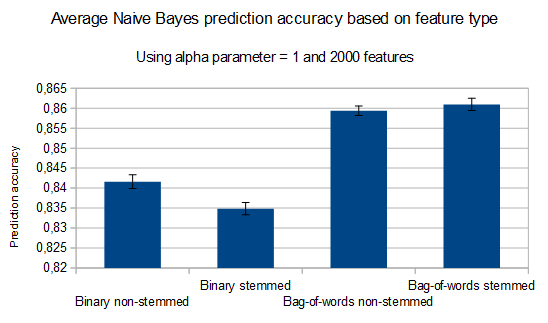
\includegraphics[width=1\columnwidth]{nb_feature_types.png}  
%\vskip 2mm
%\caption{{ \em \textbf{title}}} 
%explanation\label{fig:1}
%\centering
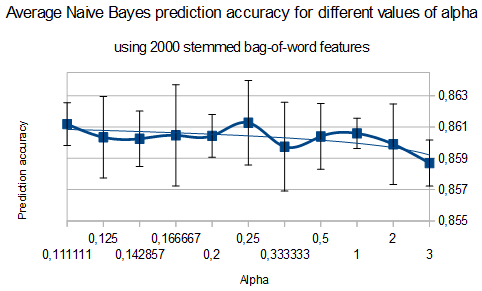
\includegraphics[width=1\columnwidth]{nb_alpha.png}  
%\vskip 2mm
%\caption{{ \em \textbf{title}}} 
%explanation\label{fig:1}
\end{figure}

\subsection{K Nearest Neighbours}

\subsection{Random Forests}
\begin{figure} 
%\centering
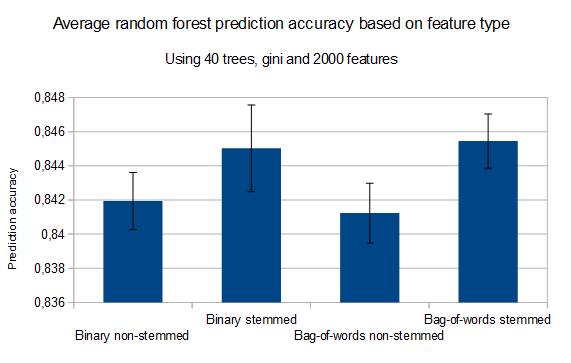
\includegraphics[width=1\columnwidth]{rf_feature_types.png}  
%\vskip 2mm
%\caption{{ \em \textbf{title}}} 
%explanation\label{fig:1}
\end{figure}

\section{Discussion}
-Combine bag-of-words with bigrams or trigrams

-Normalize the feature vectors by abstract length (here not a big difference since all abstracts are roughly the same length)

-Consider formulae (might be easy to map a given formula to a particular field!)



We hereby state that all the work presented in this report is that of the authors.

%
% The following two commands are all you need in the
% initial runs of your .tex file to
% produce the bibliography for the citations in your paper.

\bibliographystyle{abbrv}
\bibliography{sigproc}  % sigproc.bib is the name of the Bibliography in this case
% You must have a proper ".bib" file
%  and remember to run:
% latex bibtex latex latex
% to resolve all references
%
% ACM needs 'a single self-contained file'!
%
%APPENDICES are optional
%\balancecolumns

\end{document}
